\documentclass{standalone}
\usepackage{tikz}
\usepackage{ctex,siunitx}
\usepackage{tkz-euclide}
\usepackage{amsmath}
\usetikzlibrary{patterns, calc}
\usetikzlibrary {decorations.pathmorphing, decorations.pathreplacing, decorations.shapes,}
\begin{document}
\small
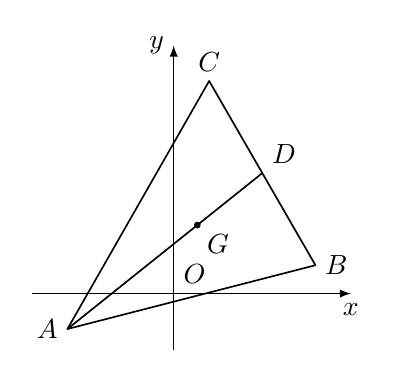
\begin{tikzpicture}[>=latex,scale=0.9]
  \draw[thin,->](-2,0)--(2.5,0)node[below]{$x$};
  \draw[thin,->](0,-0.8)--(0,3.5)node[left]{$y$};
  \tkzDefPoints{-1.5/-0.5/A,0.5/3/C,2/0.4/B,0/0/O}
  \tkzDrawPolygon[semithick](A,B,C)
  \tkzDefTriangleCenter[centroid](A,B,C)\tkzGetPoint{G}
  \tkzDefMidPoint(B,C) \tkzGetPoint{D}
  \tkzDrawPoints[fill=black](G)
  \tkzLabelPoints[left](A)
  \tkzLabelPoints[right](B)
  \tkzLabelPoints[above](C)
  \tkzLabelPoints[below right](G)
  \tkzLabelPoints[above right](O,D)
  \tkzDrawSegments[semithick](A,D)
\end{tikzpicture}
\end{document}